\documentclass{standalone}
\usepackage{tikz}
\usetikzlibrary{patterns, positioning}
\usepackage[sfdefault]{ClearSans} %% option 'sfdefault' activates Clear Sans as the default text font
\usepackage[T1]{fontenc}

\begin{document}
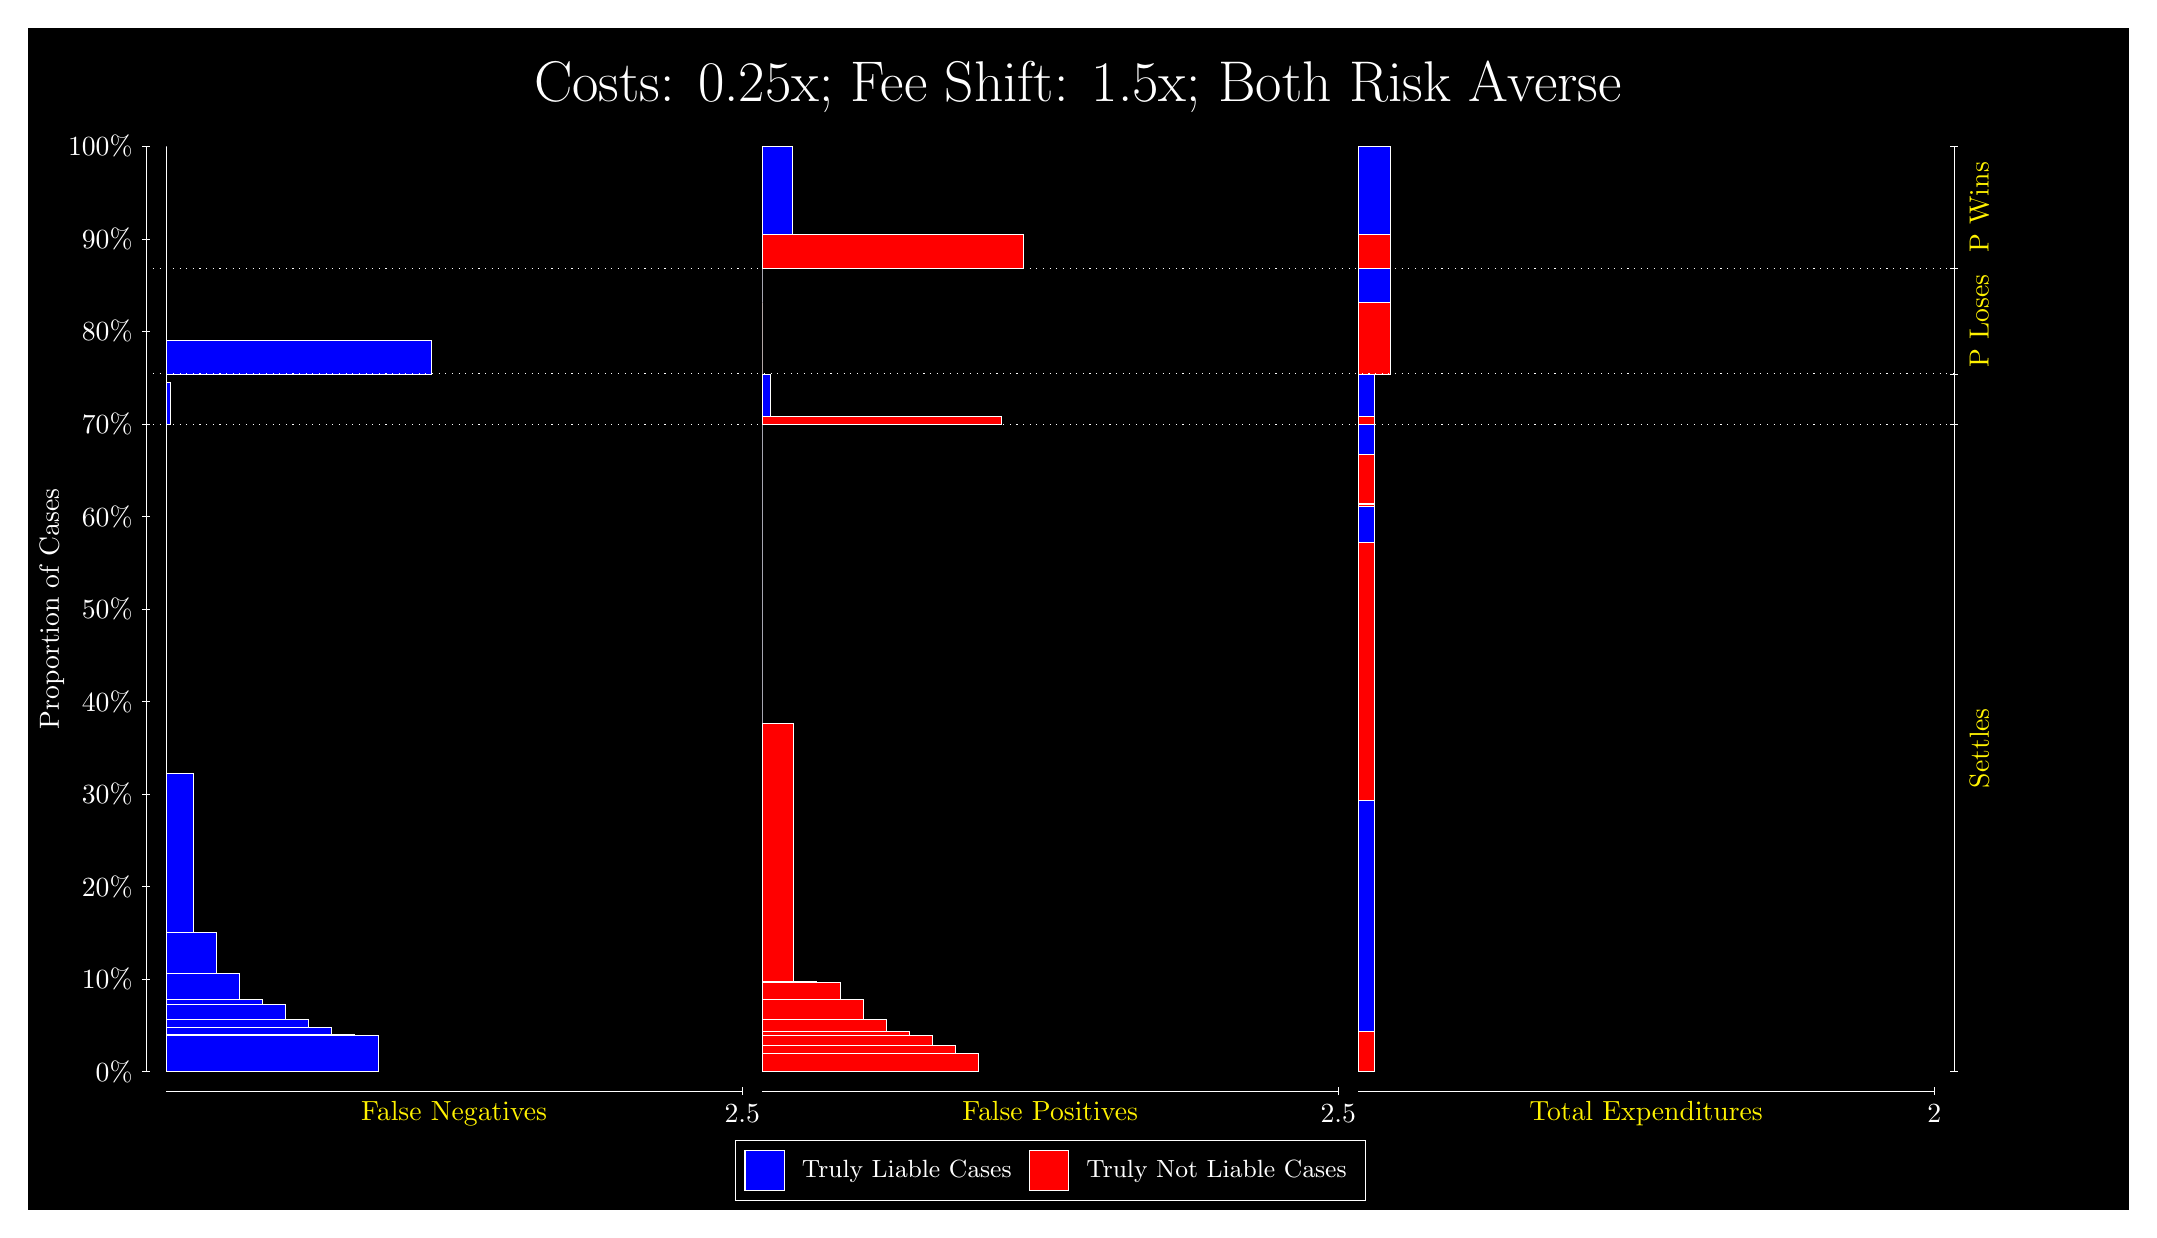
\begin{tikzpicture}
\draw[fill=black] (0,0) rectangle (26.667,15);
\draw[text=white] (0,13.5) rectangle (26.667,15) node[midway] {\huge Costs: 0.25x; Fee Shift: 1.5x; Both Risk Averse};
\draw[white, very thin] (1.5,1.75) -- (1.5,13.5);
\node[rotate=90, text=white, anchor=center] at (0.3, 7.625) {Proportion of Cases};
\draw[white, very thin] (1.45,1.75) -- (1.55,1.75);
\node[text=white, anchor=east] at (1.45, 1.75) {0\%};
\draw[white, very thin] (1.45,2.925) -- (1.55,2.925);
\node[text=white, anchor=east] at (1.45, 2.925) {10\%};
\draw[white, very thin] (1.45,4.1) -- (1.55,4.1);
\node[text=white, anchor=east] at (1.45, 4.1) {20\%};
\draw[white, very thin] (1.45,5.275) -- (1.55,5.275);
\node[text=white, anchor=east] at (1.45, 5.275) {30\%};
\draw[white, very thin] (1.45,6.45) -- (1.55,6.45);
\node[text=white, anchor=east] at (1.45, 6.45) {40\%};
\draw[white, very thin] (1.45,7.625) -- (1.55,7.625);
\node[text=white, anchor=east] at (1.45, 7.625) {50\%};
\draw[white, very thin] (1.45,8.8) -- (1.55,8.8);
\node[text=white, anchor=east] at (1.45, 8.8) {60\%};
\draw[white, very thin] (1.45,9.975) -- (1.55,9.975);
\node[text=white, anchor=east] at (1.45, 9.975) {70\%};
\draw[white, very thin] (1.45,11.15) -- (1.55,11.15);
\node[text=white, anchor=east] at (1.45, 11.15) {80\%};
\draw[white, very thin] (1.45,12.325) -- (1.55,12.325);
\node[text=white, anchor=east] at (1.45, 12.325) {90\%};
\draw[white, very thin] (1.45,13.5) -- (1.55,13.5);
\node[text=white, anchor=east] at (1.45, 13.5) {100\%};

\draw[white, very thin] (24.457,1.75) -- (24.457,13.5);
\draw[white, very thin] (24.407,1.75) -- (24.507,1.75);
\node[anchor=west] at (24.407, 1.75) {};
\draw[white, very thin] (24.407,9.9639) -- (24.507,9.9639);
\node[anchor=west] at (24.407, 9.9639) {};
\draw[white, very thin] (24.407,10.61) -- (24.507,10.61);
\node[anchor=west] at (24.407, 10.61) {};
\draw[white, very thin] (24.407,11.951) -- (24.507,11.951);
\node[anchor=west] at (24.407, 11.951) {};
\draw[white, very thin] (24.407,13.5) -- (24.507,13.5);
\node[anchor=west] at (24.407, 13.5) {};

\draw[white, very thin, fill=blue] (1.75,1.75) rectangle (4.4397,2.2097);
\draw[white, very thin, fill=blue] (1.75,2.2097) rectangle (4.1469,2.2259);
\draw[white, very thin, fill=blue] (1.75,2.2259) rectangle (3.8542,2.3077);
\draw[white, very thin, fill=blue] (1.75,2.3077) rectangle (3.5614,2.4177);
\draw[white, very thin, fill=blue] (1.75,2.4177) rectangle (3.2687,2.6019);
\draw[white, very thin, fill=blue] (1.75,2.6019) rectangle (2.9759,2.6691);
\draw[white, very thin, fill=blue] (1.75,2.6691) rectangle (2.6832,2.994);
\draw[white, very thin, fill=blue] (1.75,2.994) rectangle (2.3904,3.5159);
\draw[white, very thin, fill=blue] (1.75,3.5159) rectangle (2.0976,5.5411);
\draw[white, very thin, fill=red] (1.75,5.5411) rectangle (1.75,9.9639);
\draw[white, very thin, fill=blue] (1.75,9.9639) rectangle (1.8049,10.5);
\draw[white, very thin, fill=red] (1.75,10.5) rectangle (1.75,10.61);
\draw[white, very thin, fill=blue] (1.75,10.61) rectangle (5.1167,11.043);
\draw[white, very thin, fill=red] (1.75,11.043) rectangle (1.75,11.951);
\draw[white, very thin, fill=red] (1.75,11.951) rectangle (1.75,12.386);
\draw[white, very thin, fill=blue] (1.75,12.386) rectangle (1.75,13.5);
\draw[white, very thin, fill=red] (9.3189,1.75) rectangle (12.063,1.9795);
\draw[white, very thin, fill=red] (9.3189,1.9795) rectangle (11.771,2.0783);
\draw[white, very thin, fill=red] (9.3189,2.0783) rectangle (11.478,2.2081);
\draw[white, very thin, fill=red] (9.3189,2.2081) rectangle (11.185,2.2583);
\draw[white, very thin, fill=red] (9.3189,2.2583) rectangle (10.892,2.4185);
\draw[white, very thin, fill=red] (9.3189,2.4185) rectangle (10.6,2.6728);
\draw[white, very thin, fill=red] (9.3189,2.6728) rectangle (10.307,2.8797);
\draw[white, very thin, fill=red] (9.3189,2.8797) rectangle (10.014,2.9004);
\draw[white, very thin, fill=red] (9.3189,2.9004) rectangle (9.7214,6.1728);
\draw[white, very thin, fill=blue] (9.3189,6.1728) rectangle (9.3189,9.9639);
\draw[white, very thin, fill=red] (9.3189,9.9639) rectangle (12.356,10.073);
\draw[white, very thin, fill=blue] (9.3189,10.073) rectangle (9.4287,10.61);
\draw[white, very thin, fill=red] (9.3189,10.61) rectangle (9.3189,11.518);
\draw[white, very thin, fill=blue] (9.3189,11.518) rectangle (9.3189,11.951);
\draw[white, very thin, fill=red] (9.3189,11.951) rectangle (12.631,12.386);
\draw[white, very thin, fill=blue] (9.3189,12.386) rectangle (9.7031,13.5);
\draw[white, very thin, fill=red] (16.888,1.75) rectangle (17.094,2.2583);
\draw[white, very thin, fill=blue] (16.888,2.2583) rectangle (17.094,5.1975);
\draw[white, very thin, fill=red] (16.888,5.1975) rectangle (17.094,8.4699);
\draw[white, very thin, fill=blue] (16.888,8.4699) rectangle (17.094,8.9296);
\draw[white, very thin, fill=red] (16.888,8.9296) rectangle (17.094,8.9504);
\draw[white, very thin, fill=blue] (16.888,8.9504) rectangle (17.094,8.9666);
\draw[white, very thin, fill=red] (16.888,8.9666) rectangle (17.094,9.5879);
\draw[white, very thin, fill=blue] (16.888,9.5879) rectangle (17.094,9.9639);
\draw[white, very thin, fill=red] (16.888,9.9639) rectangle (17.094,10.073);
\draw[white, very thin, fill=blue] (16.888,10.073) rectangle (17.094,10.61);
\draw[white, very thin, fill=red] (16.888,10.61) rectangle (17.299,11.518);
\draw[white, very thin, fill=blue] (16.888,11.518) rectangle (17.299,11.951);
\draw[white, very thin, fill=red] (16.888,11.951) rectangle (17.299,12.386);
\draw[white, very thin, fill=blue] (16.888,12.386) rectangle (17.299,13.5);
\draw[white, dotted] (1.5,9.9639) -- (24.457,9.9639);
\draw[white, dotted] (1.5,10.61) -- (24.457,10.61);
\draw[white, dotted] (1.5,11.951) -- (24.457,11.951);
\draw[white, very thin] (1.75,1.5) -- (9.0689,1.5);
\node[text=yellow, anchor=north] at (5.4094, 1.5) {False Negatives};
\draw[white, very thin] (9.0689,1.45) -- (9.0689,1.55);
\node[text=white, anchor=north] at (9.0689, 1.45) {2.5};

\draw[white, very thin] (9.3189,1.5) -- (16.638,1.5);
\node[text=yellow, anchor=north] at (12.978, 1.5) {False Positives};
\draw[white, very thin] (16.638,1.45) -- (16.638,1.55);
\node[text=white, anchor=north] at (16.638, 1.45) {2.5};

\draw[white, very thin] (16.888,1.5) -- (24.207,1.5);
\node[text=yellow, anchor=north] at (20.547, 1.5) {Total Expenditures};
\draw[white, very thin] (24.207,1.45) -- (24.207,1.55);
\node[text=white, anchor=north] at (24.207, 1.45) {2};

\node[text=yellow, centered, rotate=90] at (24.777, 5.857) {Settles};

\node[text=yellow, centered, rotate=90] at (24.777, 11.28) {P Loses};
\node[text=yellow, centered, rotate=90] at (24.777, 12.726) {P Wins};

\draw (12.978300999999998,1.5) node[draw=none] (baseCoordinate) {};
\begin{scope}[align=center]
        \matrix[scale=0.5, draw=white, below=0.5cm of baseCoordinate, nodes={draw}, column sep=0.1cm]{
            \node[rectangle, draw, minimum width=0.5cm, minimum height=0.5cm, fill=blue] {}; &
            \node[draw=none, font=\small, text=white] (B) {Truly Liable Cases}; &
            \node[rectangle, draw, minimum width=0.5cm, minimum height=0.5cm, fill=red] {}; &
            \node[draw=none, font=\small, text=white] (B) {Truly Not Liable Cases}; \\
            };
\end{scope}

\end{tikzpicture}
\end{document}